\documentclass[pract,times]{SCWorks}
% Тип обучения (одно из значений):
%    bachelor   - бакалавриат (по умолчанию)
%    spec       - специальность
%    master     - магистратура
% Форма обучения (одно из значений):
%    och        - очное (по умолчанию)
%    zaoch      - заочное
% Тип работы (одно из значений):
%    coursework - курсовая работа (по умолчанию)
%    referat    - реферат
%    otchet     - универсальный отчет
%    nirjournal - журнал НИР
%    diploma    - дипломная работа
%    pract      - отчет о научно-исследовательской работе
%    autoref    - автореферат выпускной работы
%    assignment - задание на выпускную квалификационную работу
%    review     - отзыв руководителя
%    critique   - рецензия на выпускную работу
% Включение шрифта
%    times      - включение шрифта Times New Roman (если установлен)
%                 по умолчанию выключен
\usepackage{preamble}

\begin{document}

% Кафедра (в родительном падеже)
\chair{информатики и программирования}

% Тема работы
\title{Теория графов}

% Курс
\course{3}

% Группа
\group{351}

% Факультет (в родительном падеже) (по умолчанию "факультета КНиИТ")
% \department{факультета КНиИТ}

% Специальность/направление код - наименование
% \napravlenie{02.03.02 "--- Фундаментальная информатика и информационные технологии}
% \napravlenie{02.03.01 "--- Математическое обеспечение и администрирование информационных систем}
% \napravlenie{09.03.01 "--- Информатика и вычислительная техника}
\napravlenie{09.03.04 "--- Программная инженерия}
% \napravlenie{10.05.01 "--- Компьютерная безопасность}

% Для студентки. Для работы студента следующая команда не нужна.
% \studenttitle{Студентки}

% Фамилия, имя, отчество в родительном падеже
\author{Мангасаряна Евгения Павловича}

% Заведующий кафедрой
\chtitle{доцент, к.\,ф.-м.\,н.} % степень, звание
\chname{М.\,В.\,Огнева}

% Научный руководитель (для реферата преподаватель проверяющий работу)
\satitle{доцент} %должность, степень, звание
\saname{А.\,П.\,Грецова}

% Семестр (только для практики, для остальных типов работ не используется)
\term{1}

% Наименование практики (только для практики, для остальных типов работ не
% используется)
\practtype{учебная (рассредоточенная)}

% Год выполнения отчета
\date{2023}

\maketitle

% Включение нумерации рисунков, формул и таблиц по разделам (по умолчанию -
% нумерация сквозная) (допускается оба вида нумерации)
\secNumbering

\tableofcontents

\intro
Целью практической работы является закрепление и углубление теоретических знаний по 
дисциплине <<Теория графов>> посредством реализации класса
<<Граф>> на выбранном языке программирования.
Для достижения данной цели были поставлены следующие задачи:
\begin{itemize}
  \item создание класса <<Граф>>;
  \item работа со cписками смежности;
  \item реализация обходов графа;
  \item построение минимального остовного дерева;
  \item работа со взвешенным графом;
  \item реализация потокового алгоритма;
  \item выполнение творческого задания.
\end{itemize}
Все задачи выполнены с использованием языка программирования TypeScript.

\section{Минимальные требования для класса <<Граф>>}
\subsection{Условие задания}
Для решения всех задач курса необходимо создать класс (или иерархию
классов "--- на усмотрение разработчика), содержащий:
\begin{enumerate}
  \item Структуру для хранения списка смежности графа (не работать с графом
  через матрицы смежности, если в некоторых алгоритмах удобнее использовать
  список ребер "--- реализовать метод, создающий список ребер на
  основе списка смежности).
  \item Конструкторы (не менее 3"~х):
  \begin{itemize}
    \item добавляющие вершину;
    \item добавляющие ребро (дугу);
    \item удаляющие вершину;
    \item удаляющие ребро (дугу);
    \item выводящие список смежности в файл (в том числе в пригодном для
    чтения конструктором формате).
  \end{itemize}
  \item Методы:
  \begin{itemize}
    \item конструктор по умолчанию, создающий пустой граф;
    \item конструктор, заполняющий данные графа из файла;
    \item конструктор"=копию (аккуратно, не все сразу делают именно копию);
    \item специфические конструкторы для удобства тестирования.
  \end{itemize}
  \item Должны поддерживаться как ориентированные, так и неориентированные
  графы.
  \item Добавьте минималистичный консольный интерфейс пользователя, позволяющий
  добавлять и удалять вершины и ребра (дуги) и просматривать
  текущий список смежности графа.
\end{enumerate}

\subsection{Примеры исходного кода}
Следующий код описывает класс \mitext{Graph}, соответствующий требованиям
условия:
\begin{minted}{typescript}
export class Graph {
  private adj: Map<string, Map<string, number>> = new Map()
  private weighted: boolean = false
  private oriented: boolean = false

  constructor(weighted: boolean, oriented: boolean)
  constructor(textRepr: string)
  constructor(other: Graph)
  constructor(arg1: boolean | string | Graph, arg2?: boolean) {
    if (typeof arg1 === 'boolean' && typeof arg2 === 'boolean') {
      this.weighted = arg1
      this.oriented = arg2
      this.adj = new Map()
    } else if (typeof arg1 === 'string' && arg2 == null) {
      this.loadFromFile(arg1)
      if (!this.oriented) {
        for (const [v, neighbors] of this.adj) {
          for (const [u, w] of neighbors) {
            this.adj.get(u)!.set(v, w)
          }
        }
      }
    } else if (arg1 instanceof Graph && arg2 == null) {
      this.weighted = arg1.weighted
      this.oriented = arg1.oriented
      this.adj = new Map(arg1.adj)
    } else {
      throw new Error('Invalid arguments')
    }
  }
  // другие методы ...
}
\end{minted}

Методы для добавления вершины и ребра (дуги):
\begin{minted}{typescript}
addNode(label: string) {
  if (this.adj.has(label)) {
    throw new NodeAlreadyExists(label)
  }
  this.adj.set(label, new Map())
}

connect(a: string, b: string, weight?: number) {
  if (!this.adj.has(a)) {
    throw new NodeNotExists(a)
  }
  if (!this.adj.has(b)) {
    throw new NodeNotExists(b)
  }
  if (this.adj.get(a)!.has(b)) {
    throw new ConnectionAlreadyExists(a, b)
  }

  if (this.weighted) {
    this.adj.get(a)!.set(b, weight!)
    if (!this.oriented) {
      this.adj.get(b)!.set(a, weight!)
    }
  } else {
    if (weight) {
      throw new WeightsInNonWeightedGraph()
    }
    this.adj.get(a)!.set(b, 0)
    if (!this.oriented) {
      this.adj.get(b)!.set(a, 0)
    }
  }
}
\end{minted}

Удаление вершины и дуги (ребра):
\begin{minted}{typescript}
removeNode(label: string) {
  if (!this.adj.has(label)) {
    throw new NodeNotExists(label)
  }

  this.adj.delete(label)
  for (let value of this.adj.values()) {
    value.delete(label)
  }
}

disconnect(a: string, b: string) {
  if (!this.adj.has(a)) {
    throw new NodeNotExists(a)
  }
  if (!this.adj.has(b)) {
    throw new NodeNotExists(b)
  }
  if (!this.adj.get(a)!.has(b)) {
    throw new ConnectionNotExists(a, b)
  }

  this.adj.get(a)!.delete(b)
  if (!this.oriented) {
    this.adj.get(b)!.delete(a)
  }
}
\end{minted}

Вместо консольного сразу был реализован веб"=интерфейс на React.js.
Основной компонент интерфейса (\mitext{App}) представлен в приложении
\ref{app:app-component}.

\subsection{Примеры входных и выходных данных}
Взвешенный ориентированный граф:
\begin{minted}{js}
{
  "weighted": true,
  "oriented": true,
  "adj": {
    "a": {
      "b": 2,
      "c": 3
    },
    "b": {
      "d": 5
    },
    "c": {
      "e": 4,
      "f": 2
    },
    "d": {
      "g": 6
    },
    "e": {
      "h": 3
    },
    "f": {
      "h": 7
    },
    "g": {
      "h": 8
    },
    "h": {}
  }
}
\end{minted}

Взвешенный неориентированный граф:
\begin{minted}{js}
{
  "weighted": true,
  "oriented": false,
  "adj": {
    "a": {
      "b": 2,
      "c": 3,
      "d": 5
    },
    "b": {
      "c": 4,
      "e": 6
    },
    "c": {
      "d": 1,
      "f": 3
    },
    "d": {
      "g": 2
    },
    "e": {
      "f": 4,
      "h": 5
    },
    "f": {
      "h": 2,
      "g": 3
    },
    "g": {
      "h": 1
    },
    "h": {}
  }
}
\end{minted}

Выходные файлы имеют такой же формат и полностью совместимы с входными.

\section{Список смежности Ia}
\subsection{Условие задания}
\textbf{Вариант 5:} Для каждой вершины орграфа вывести её степень.

\subsection{Примеры исходного кода}
Для нахождения и вывода степени каждой вершины был создан вспомогательный
компонент \mitext{VertexPowers}, который находит степени вершин и выводит
их в виде таблицы:
\begin{minted}{jsx}
function VertexPowers() {
  const adjList = graph.current!.getAdjacencyList()
  const powers = new Map()

  for (const [k, v] of adjList) {
    powers.set(k, v.length)
    for (const [otherK, otherV] of adjList) {
      if (k === otherK) continue

      if (otherV.find(value => value[0] === k)) {
        powers.set(k, powers.get(k) + 1)
      }
    }
  }

  return (
    <TableBody>
      {graph.current!.getAdjacencyList().map(item => {
        return (
          <TableRow key={item[0]}>
            <TableCell align='right'>{item[0]}</TableCell>
            <TableCell align='left'>{powers.get(item[0])}</TableCell>
          </TableRow>
        )
      })
      }
    </TableBody>
  )
}
\end{minted}

\subsection{Краткое описание алгоритма}
Для каждой вершины подсчитывается степень исхода и степень захода,
а затем суммируются.

\subsection{Примеры входных и выходных данных}
\subsubsection{Входные данные}
\begin{figure}[H]
  \begin{minipage}{0.5\textwidth}
    \centering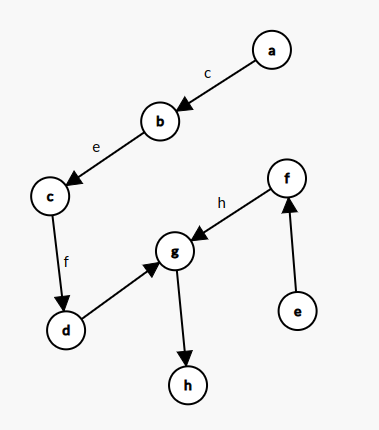
\includegraphics[width=\linewidth]{figs/task-2/graph-1.png}
  \end{minipage}
  \begin{minipage}{0.5\textwidth}
    \centering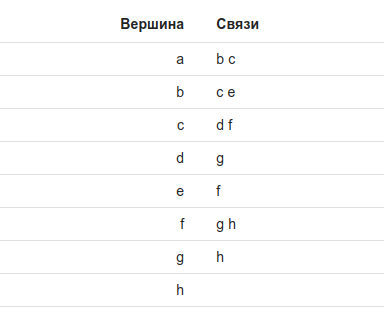
\includegraphics[width=\linewidth]{figs/task-2/adj-1.png}
  \end{minipage}
  \caption{Ориентированный граф}
\end{figure}

\begin{minted}{js}
{
  "weighted": false,
  "oriented": true,
  "adj": {
    "a": {
      "b": 0,
      "c": 0
    },
    "b": {
      "c": 0,
      "e": 0
    },
    "c": {
      "d": 0,
      "f": 0
    },
    "d": {
      "g": 0
    },
    "e": {
      "f": 0
    },
    "f": {
      "g": 0,
      "h": 0
    },
    "g": {
      "h": 0
    },
    "h": {}
  }
}
\end{minted}

\subsubsection{Выходные данные}
\begin{figure}[H]
  \centering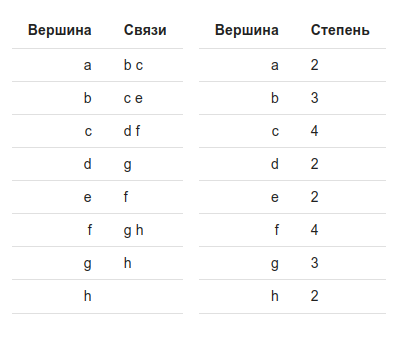
\includegraphics[width=0.5\textwidth]{figs/task-2/res-1.png}
  \caption{Результат работы}
\end{figure}
\section{Список смежности Ia}
\subsection{Условие задания}
\textbf{Вариант 20:} Вывести все вершины орграфа, не смежные с данной.

\subsection{Примеры исходного кода}
Для нахождения и вывода вершин орграфа, не смежных с данной, был
описан метод \mitext{getAdjacent()}:
\begin{minted}{typescript}
getAdjacent(label: string): Map<string, number> {
  if (!this.adj.has(label)) {
    throw new NodeNotExists(label)
  }
  return this.adj.get(label)!
}
\end{minted}

Затем, при выводе результата, запрашиваются все метки вершин орграфа и
из них отбрасываются те, которые смежны с данной:
\begin{minted}{typescript}
let resList: string[] = []
for (const [node, _] of graph.current!.getAdjacencyList()) {
  if (nodeName !== node && !adj.has(node)) {
    resList.push(node.toString())
  }
}
setAnswer(resList.join(', '))
\end{minted}

\subsection{Краткое описание алгоритма}
Поскольку данные о смежности хранятся в виде списка смежности, достаточно
для заданной вершины запросить информацию о смежных с ней вершинах.
А далее простая фильтрация списка строк.

Поскольку графы могут быть взвешенными, и как пересекать веса не оговаривается,
то выбирается минимум из двух весов при пересечении.

\subsection{Примеры входных и выходных данных}
\subsubsection{Входные данные}
\begin{figure}[H]
  \begin{minipage}{0.5\textwidth}
    \centering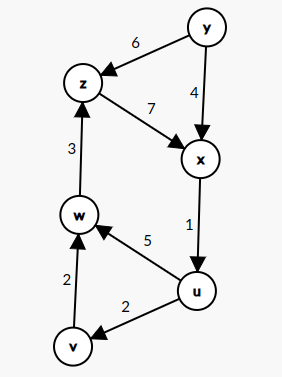
\includegraphics[width=0.6\linewidth]{figs/task-3/graph-2.png}
  \end{minipage}
  \begin{minipage}{0.5\textwidth}
    \centering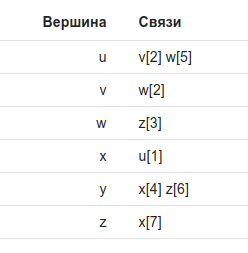
\includegraphics[width=0.6\linewidth]{figs/task-3/adj-2.png}
  \end{minipage}
  \caption{Ориентированный граф}
\end{figure}

\begin{minted}{js}
{
  "weighted": true,
  "oriented": true,
  "adj": {
    "u": {
      "v": 2,
      "w": 5
    },
    "v": {
      "w": 2
    },
    "w": {
      "z": 3
    },
    "x": {
      "u": 1
    },
    "y": {
      "x": 4,
      "z": 6
    },
    "z": {
      "x": 7
    }
  }
}
\end{minted}

\subsubsection{Выходные данные}
\begin{figure}[H]
  \centering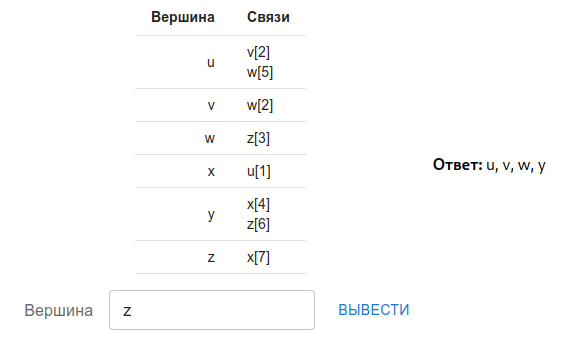
\includegraphics[width=0.8\textwidth]{figs/task-3/res-2.png}
  \caption{Результат работы}
\end{figure}
\section{Список смежности Iб: несколько графов}
\subsection{Условие задания}
\textbf{Вариант 8:} Построить орграф, являющийся пересечением двух заданных.

\subsection{Примеры исходного кода}
Для нахождения пересечения двух орграфов был описан метод \mitext{intersect()}:
\begin{minted}{typescript}
intersect(other: Graph): Graph {
  if (!this.oriented || !other.oriented) {
    throw new InvalidOperandTypes()
  }

  const res = new Graph(this.weighted || other.weighted, true)
  const intersection = new Map<string, Map<string, number>>()

  const commonNodes = Array.from(this.adj.keys()).filter(node => other.adj.has(node))

  for (const node of commonNodes) {
    const neighborsA = this.adj.get(node) || new Map<string, number>()
    const neighborsB = other.adj.get(node) || new Map<string, number>()
    const commonNeighbors = new Map<string, number>()

    for (const [neighbor, weightA] of neighborsA) {
      if (neighborsB.has(neighbor)) {
        const weightB = neighborsB.get(neighbor) || 0
        commonNeighbors.set(neighbor, Math.min(weightA, weightB))
      }
    }

    intersection.set(node, commonNeighbors)
  }

  res.adj = intersection
  return res
}
\end{minted}

В интерфейсе орграф"=пересечение выводится как обычно, в виде списка смежности.

\subsection{Краткое описание алгоритма}
Создается новый граф, в котором будет накапливаться результат. Затем
по определению "--- добавляем в результат только нужные вершины и дуги.

\subsection{Примеры входных и выходных данных}
\subsubsection{Входные данные}
\begin{figure}[H]
  \begin{minipage}{0.5\textwidth}
    \centering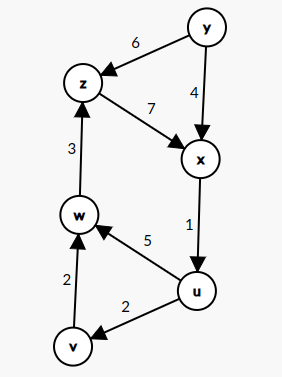
\includegraphics[width=0.6\linewidth]{figs/task-4/graph-3.png}
  \end{minipage}
  \begin{minipage}{0.5\textwidth}
    \centering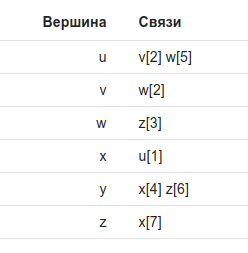
\includegraphics[width=0.6\linewidth]{figs/task-4/adj-3.png}
  \end{minipage}
  \caption{Первый ориентированный граф}
\end{figure}

\begin{figure}[H]
  \begin{minipage}{0.5\textwidth}
    \centering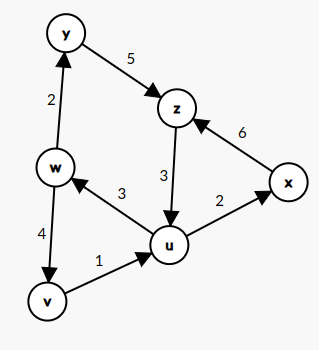
\includegraphics[width=0.6\linewidth]{figs/task-4/graph-4.png}
  \end{minipage}
  \begin{minipage}{0.5\textwidth}
    \centering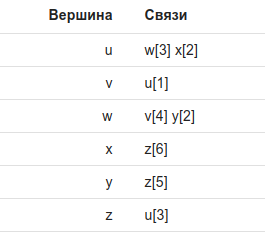
\includegraphics[width=0.6\linewidth]{figs/task-4/adj-4.png}
  \end{minipage}
  \caption{Второй ориентированный граф}
\end{figure}

\begin{minipage}{0.5\textwidth}
  \begin{minted}{js}
// первый орграф
{
  "weighted": true,
  "oriented": true,
  "adj": {
    "u": {
      "w": 3,
      "x": 2
    },
    "v": {
      "u": 1
    },
    "w": {
      "v": 4,
      "y": 2
    },
    "x": {
      "z": 6
    },
    "y": {
      "z": 5
    },
    "z": {
      "u": 3
    }
  }
}
  \end{minted}
\end{minipage}
\begin{minipage}{0.5\textwidth}
  \begin{minted}{js}
// второй орграф
{
  "weighted": true,
  "oriented": true,
  "adj": {
    "u": {
      "v": 2,
      "w": 5
    },
    "v": {
      "w": 2
    },
    "w": {
      "z": 3
    },
    "x": {
      "u": 1
    },
    "y": {
      "x": 4,
      "z": 6
    },
    "z": {
      "x": 7
    }
  }
}
  \end{minted}
\end{minipage}

\subsubsection{Выходные данные}
\begin{figure}[H]
  \begin{minipage}{0.5\textwidth}
    \centering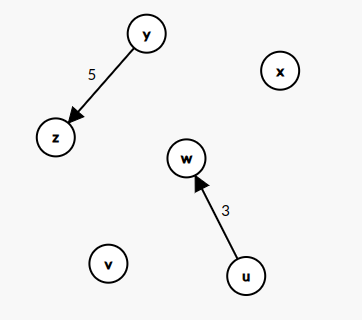
\includegraphics[width=0.8\linewidth]{figs/task-4/res-graph-4.png}
  \end{minipage}
  \begin{minipage}{0.5\textwidth}
    \centering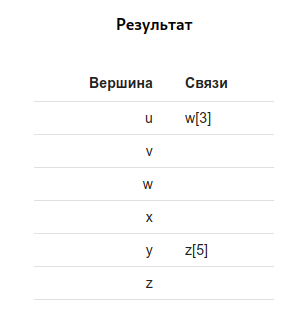
\includegraphics[width=0.8\linewidth]{figs/task-4/res-4.png}
  \end{minipage}
  \caption{Результат работы}
\end{figure}
\section{Обходы графа II}
\subsection{Условие задания}
\textbf{Вариант 5:} Подсчитать количество связных компонент графа.

\subsection{Примеры исходного кода}
Для нахождения компонент связности графа был описан метод\\
\mitext{connectedComponents()}:
\begin{minted}{typescript}
connectedComponents(): number {
  const visited: Set<string> = new Set()

  let count = 0 // количество компонент
  for (const node of this.adj.keys()) {
    if (!visited.has(node)) { // если еще не посетили, выполнить DFS
      count++ // новая компонента
      this.dfs(node, visited) // DFS посещаем все узлы в этой компоненте связности
    }
  }

  return count
}
\end{minted}

А также вспомогательный метод обхода в глубину:
\begin{minted}{typescript}
private dfs(node: string, visited: Set<string>) {
  visited.add(node)

  const neighbors = this.adj.get(node)!
  for (const neighbor of neighbors.keys()) {
    if (!visited.has(neighbor)) {
      this.dfs(neighbor, visited) // рекурсивно обойти соседние узлы
    }
  }
}
\end{minted}

\subsection{Краткое описание алгоритма}
Вводится счетчик количества компонент связности. Также ведется множество
уже посещенных вершин. Алгоритм заканчивает работу, когда все вершины посещены.
На каждой итерации выбирается непосещенная вершина и с помощью обхода
в глубину посещаются все связные с ней вершины (одна компонента связности).
Таким образом, мы сможем подсчитать, сколько всего компонент связности
в графе.

\subsection{Примеры входных и выходных данных}
\subsubsection{Входные данные}
\begin{figure}[H]
  \begin{minipage}{0.5\textwidth}
    \centering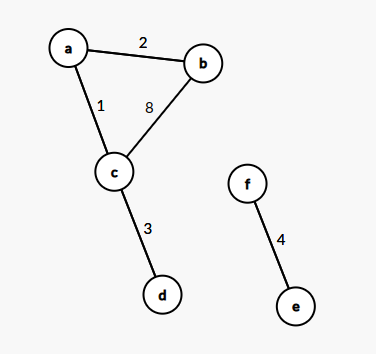
\includegraphics[width=0.6\linewidth]{figs/task-5/graph-5.png}
  \end{minipage}
  \begin{minipage}{0.5\textwidth}
    \centering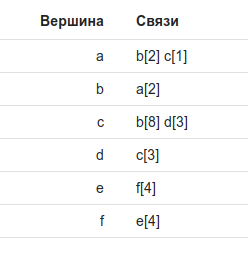
\includegraphics[width=0.6\linewidth]{figs/task-5/adj-5.png}
  \end{minipage}
  \caption{Неориентированный граф}
\end{figure}

\begin{minted}{js}
{
  "weighted": true,
  "oriented": false,
  "adj": {
    "a": {
      "b": 2,
      "c": 1
    },
    "b": {
      "a": 2
    },
    "c": {
      "a": 1,
      "d": 3
    },
    "d": {
      "c": 3
    },
    "e": {
      "f": 4
    },
    "f": {
      "e": 4
    }
  }
}
\end{minted}

\subsubsection{Выходные данные}
\begin{figure}[H]
  \centering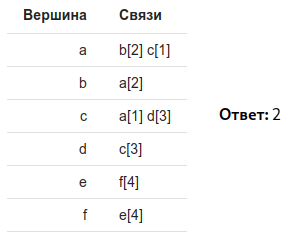
\includegraphics[width=0.4\textwidth]{figs/task-5/res-5.png}
  \caption{Результат работы}
\end{figure}
\section{Обходы графа II}
\subsection{Условие задания}
\textbf{Вариант 27:} Найти длины кратчайших (по числу дуг) путей из вершины $u$ во все остальные.

\subsection{Примеры исходного кода}
Для нахождения длины кратчайших путей из вершины $u$ во все остальные
был объявлен метод \mitext{shortestPathLengthsFrom()}, принимающий
метку вершины $u$ и возвращающий расстояния до всех вершин графа (по числу дуг):
\begin{minted}{typescript}
shortestPathLengthsFrom(u: string): Map<string, number> {
  if (!this.adj.has(u)) {
    throw new NodeNotExists(u)
  }

  const shortestPaths: Map<string, number> = new Map()

  for (const node of this.adj.keys()) {
    shortestPaths.set(node, Infinity) // пока считаем, что расстояния до других узлов бесконечность
  }
  shortestPaths.set(u, 0) // расстояние до самого себя 0

  const queue = [u] // очередь обхода
  while (queue.length > 0) {
    const currentNode = queue.shift()!
    const neighbors = this.adj.get(currentNode)!

    for (const neighbor of neighbors.keys()) {
      if (shortestPaths.get(neighbor) === Infinity) { // если узел еще не был посещен
        // установить кратчайшее расстояние до него
        shortestPaths.set(neighbor, shortestPaths.get(currentNode)! + 1)
        queue.push(neighbor) // добавить соседний узел в очередь обхода
      }
    }
  }

  return shortestPaths
}
\end{minted}

\subsection{Краткое описание алгоритма}
Этот алгоритм использует метод обхода в ширину (BFS) для нахождения кратчайших путей.

Создается \mitext{Map<string, number>}, где для каждой вершины устанавливается начальное расстояние.
Расстояние от $u$ до самой себя равно $0$, а до остальных вершин "--- бесконечность.

Используется очередь для обхода графа. Начальная вершина $u$ добавляется в очередь.
Пока очередь не пуста, извлекается текущая вершина. Для каждого соседнего узла проверяется,
был ли он уже посещен. Если не был, устанавливается кратчайшее расстояние и добавляется в очередь.

\subsection{Примеры входных и выходных данных}
\subsubsection{Входные данные}
\begin{figure}[H]
  \begin{minipage}{0.5\textwidth}
    \centering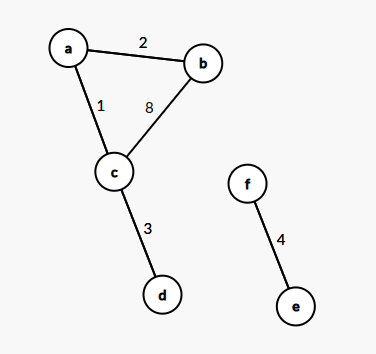
\includegraphics[width=0.6\linewidth]{figs/task-6/graph-6.png}
  \end{minipage}
  \begin{minipage}{0.5\textwidth}
    \centering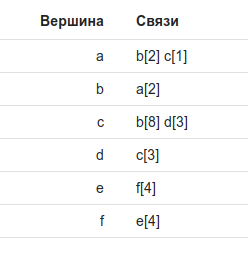
\includegraphics[width=0.6\linewidth]{figs/task-6/adj-6.png}
  \end{minipage}
  \caption{Неориентированный граф}
\end{figure}

\begin{minted}{js}
{
  "weighted": true,
  "oriented": false,
  "adj": {
    "a": {
      "b": 2,
      "c": 1
    },
    "b": {
      "a": 2
    },
    "c": {
      "a": 1,
      "d": 3
    },
    "d": {
      "c": 3
    },
    "e": {
      "f": 4
    },
    "f": {
      "e": 4
    }
  }
}
\end{minted}

\subsubsection{Выходные данные}
\begin{figure}[H]
  \centering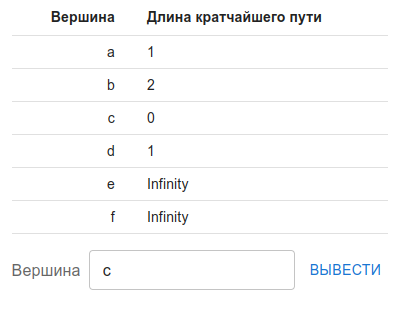
\includegraphics[width=0.4\textwidth]{figs/task-6/res-6.png}
  \caption{Результат работы}
\end{figure}
\section{Каркас III}
\subsection{Условие задания}
Дан взвешенный неориентированный граф из $N$ вершин и $M$ ребер.
Требуется найти в нем каркас минимального веса. (Алгоритм Прима)

\subsection{Примеры исходного кода}
Для нахождения каркаса минимального веса взвешенного неориентированного
графа был создан метод \mitext{mst()} (\textit{Minimal Spanning Tree}):
\begin{minted}{typescript}
mst(): Graph {
  if (!this.weighted || this.oriented) {
    throw new GraphNotWeightedUnoriented()
  }

  const mst = new Graph(true, false) // минимальное остовное дерево
  const visited = new Set<string>() // множество посещенных вершин

  // взять любую вершину как начальную (здесь первая)
  const startVertex = this.adj.keys().next().value
  if (!startVertex) {
    throw new GraphIsEmpty()
  }
  visited.add(startVertex)
  mst.addNode(startVertex)

  while (visited.size < this.adj.size) { // пока не посетим все вершины
    // ребра, которые соединяют посещенные вершины с непосещенными
    const edges: Array<Edge> = []

    for (const vertex of visited) { // найти такие ребра
      for (const [neighbor, weight] of this.adj.get(vertex)!) {
        if (!visited.has(neighbor)) {
          edges.push({from: vertex, to: neighbor, weight});
        }
      }
    }

    if (edges.length === 0) {
      // Не все вершины еще посещены, но мы не смогли найти новые ребра.
      // Это значит, что граф несвязный.
      throw new GraphIsNotConnected()
    }

    // выбрать ребро с наименьшим весом
    edges.sort((a, b) => a.weight - b.weight)
    const {from, to, weight} = edges[0]

    // добавить ребро в минимальное остовное дерево
    mst.addNode(to)
    mst.connect(from, to, weight)
    visited.add(to)
  }

  return mst
}
\end{minted}

\subsection{Краткое описание алгоритма}
Основная идея заключается в том, чтобы начать с одной вершины и пошагово добавлять ребра
минимального веса, соединяющие посещенные вершины с непосещенными.

Создается новый граф \mitext{mst}, представляющий минимальное остовное дерево.
Также создается множество \mitext{visited} для отслеживания посещенных вершин.
Выбирается любая вершина в качестве начальной. В данной реализации используется
первая вершина из списка вершин графа.

Пока не посещены все вершины графа, выполняется цикл:
\begin{enumerate}
  \item Создается массив \mitext{edges}, содержащий ребра, соединяющие посещенные вершины с непосещенными.
  \item Если массив \mitext{edges} пуст, это означает, что граф несвязный (ошибка).
  \item Ребра в массиве сортируются по весу, и выбирается ребро с минимальным весом.
  \item Выбранное ребро добавляется в остовное дерево, связывая вершины \mitext{from} и \mitext{to} с весом
  \mitext{weight}. Вершина \mitext{to} помечается как посещенная.
\end{enumerate}

\subsection{Примеры входных и выходных данных}
\subsubsection{Входные данные}
\begin{figure}[H]
  \begin{minipage}{0.5\textwidth}
    \centering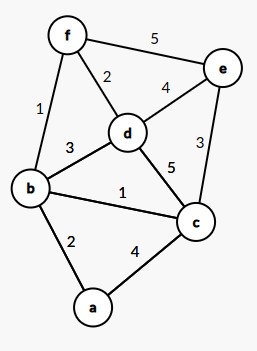
\includegraphics[width=0.6\linewidth]{figs/task-7/graph-7.png}
  \end{minipage}
  \begin{minipage}{0.5\textwidth}
    \centering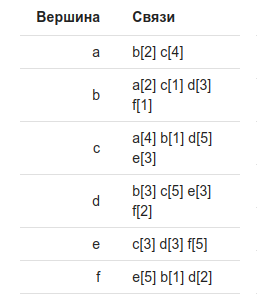
\includegraphics[width=0.6\linewidth]{figs/task-7/adj-7.png}
  \end{minipage}
  \caption{Неориентированный взвешенный граф}
\end{figure}

\begin{minted}{js}
{
  "weighted": true,
  "oriented": false,
  "adj": {
    "a": {
      "b": 2,
      "c": 4
    },
    "b": {
      "a": 2,
      "c": 1,
      "d": 3,
      "f": 1
    },
    "c": {
      "a": 4,
      "b": 1,
      "d": 5,
      "e": 3
    },
    "d": {
      "b": 3,
      "c": 5,
      "e": 3,
      "f": 2
    },
    "e": {
      "c": 3,
      "d": 4,
      "f": 5
    },
    "f": {
      "e": 5,
      "b": 1,
      "d": 2
    }
  }
}
\end{minted}

\subsubsection{Выходные данные}
\begin{figure}[H]
  \begin{minipage}{0.5\textwidth}
    \centering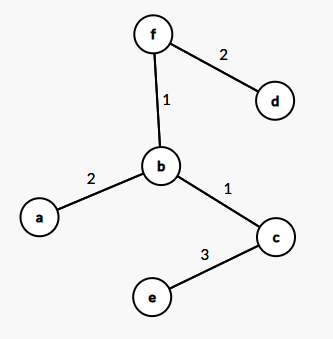
\includegraphics[width=0.8\linewidth]{figs/task-7/res-graph-7.png}
  \end{minipage}
  \begin{minipage}{0.5\textwidth}
    \centering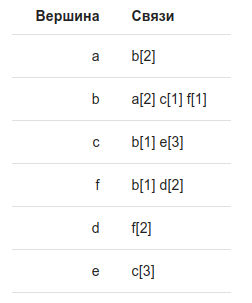
\includegraphics[width=0.6\linewidth]{figs/task-7/res-7.png}
  \end{minipage}
  \caption{Результат работы}
\end{figure}
\section{Веса IV а}
\subsection{Условие задания}
В графе нет ребер отрицательного веса.

\textbf{Вариант 2:} Определить, есть ли в графе вершина, минимальные стоимости путей от
которой до остальных в сумме не превосходят P.

\subsection{Примеры исходного кода}
Для этой задачи был создан метод \mitext{taskEight()}::
\begin{minted}{typescript}
/**
 * Метод, определяющий, есть ли в графе вершина такая, что сумма
 * длин кратчайших путей от нее до всех остальных вершин
 * не превышает `P`. Построен на основе алгоритма Дейкстры.
 * В графе не может быть отрицательных весов.
 * @param P
 */
taskEight(P: number): boolean {
  /**
   * Вспомогательная функция для определения вершины, до которой
   * путь кратчайший. Возвращает `null`, если пути вообще нет.
   * @param dist расстояния до других вершин
   * @param visited множество посещенных
   */
  const minDistance = (dist: Map<string, number>, visited: Set<string>): string | null => {
    let min = Infinity  // минимальное расстояние
    let minVertex: string | null = null  // метка вершины, до которой расстояние минимальное

    for (const vertex of this.adj.keys()) {
      if (!visited.has(vertex) && dist.get(vertex)! <= min) {
        min = dist.get(vertex)!
        minVertex = vertex
      }
    }

    return minVertex
  }

  /**
   * Алгоритм Дейкстры нахождения кратчайших путей.
   * @param source начальная вершина
   */
  const dijkstra = (source: string): Map<string, number> => {
    const dist: Map<string, number> = new Map()  // расстояния до других вершин
    const visited: Set<string> = new Set()  // для контроля уже посещенных вершин

    // инициализируем расстояния бесконечностью
    for (const vertex of this.adj.keys()) {
      dist.set(vertex, Infinity)
    }

    dist.set(source, 0)  // расстояние до самой себя 0

    for (let i = 0; i < this.adj.size - 1; i++) {
      const u = minDistance(dist, visited)
      if (u === null) {
        break  // если нет путей в непосещенные вершины
      }

      visited.add(u)

      for (const [v, weight] of this.adj.get(u)!.entries()) {
        if (weight < 0) {
          throw new GraphHasNegativeWeights()
        }

        const newDist = dist.get(u)! + weight
        if (newDist < dist.get(v)!) {
          dist.set(v, newDist)
        }
      }
    }

    return dist
  }

  // вычислить сумму длин кратчайших путей для каждой вершины
  for (const vertex of this.adj.keys()) {
    const dist = dijkstra(vertex)
    const sum = Array.from(dist.values())
      .reduce((acc, val) => acc + val, 0)

    if (sum > P) {
      return false
    }
  }

  return true
}
\end{minted}

\subsection{Краткое описание алгоритма}
Алгоритм основан на модификации алгоритма Дейкстры для нахождения кратчайших путей во
взвешенных неориентированных графах.

Вспомогательная функция \mitext{minDistance()}
находит вершину, до которой кратчайшее расстояние и возвращает ее метку.
В случае отсутствия путей в непосещенные вершины возвращает \mitext{null}.

Для каждой вершины графа выполняется алгоритм Дейкстры, который находит кратчайшие
пути от этой вершины до всех остальных. Веса ребер проверяются на отрицательность,
так как алгоритм Дейкстры не будет корректно работать в этом случае.

После нахождения кратчайших путей для каждой вершины вычисляется сумма длин этих
путей. Если сумма превышает заданное значение \mitext{P}, алгоритм возвращает \mitext{false},
иначе \mitext{true}.

\subsection{Примеры входных и выходных данных}
\subsubsection{Входные данные}
\begin{figure}[H]
  \begin{minipage}{0.5\textwidth}
    \centering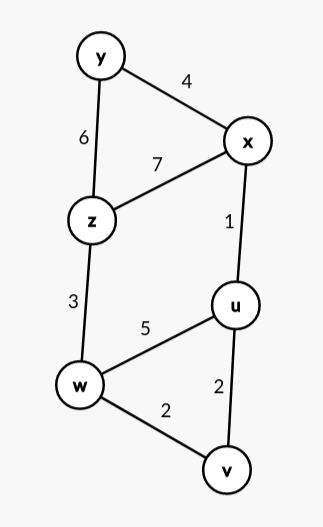
\includegraphics[width=0.6\linewidth]{figs/task-8/graph-8.png}
  \end{minipage}
  \begin{minipage}{0.5\textwidth}
    \centering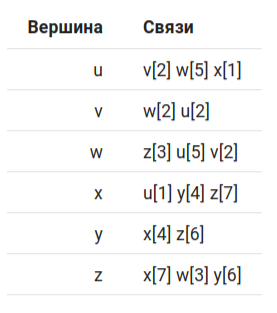
\includegraphics[width=0.6\linewidth]{figs/task-8/adj-8.png}
  \end{minipage}
  \caption{Взвешенный граф}
\end{figure}

\begin{minted}{js}
{
  "weighted": true,
  "oriented": false,
  "adj": {
    "u": {
      "v": 2,
      "w": 5
    },
    "v": {
      "w": 2
    },
    "w": {
      "z": 3
    },
    "x": {
      "u": 1
    },
    "y": {
      "x": 4,
      "z": 6
    },
    "z": {
      "x": 7
    }
  }
}
\end{minted}

\subsubsection{Выходные данные}
\begin{figure}[H]
  \begin{minipage}{0.5\textwidth}
    \centering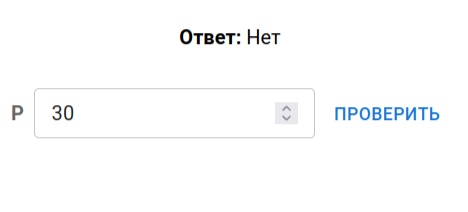
\includegraphics[width=0.8\linewidth]{figs/task-8/res-8-1.png}
  \end{minipage}
  \begin{minipage}{0.5\textwidth}
    \centering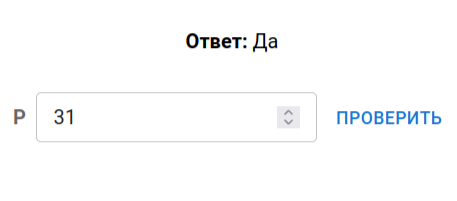
\includegraphics[width=0.8\linewidth]{figs/task-8/res-8-2.png}
  \end{minipage}
  \caption{Результат работы}
\end{figure}
\section{Веса IV b}
\subsection{Условие задания}
В графе нет циклов отрицательного веса.

\textbf{Вариант 14:} 
Вывести кратчайшие пути из вершины $u$ во все остальные вершины.

\subsection{Примеры исходного кода}
Для выполнения задания был реализован метод\\
\mitext{taskNine()}:
\begin{minted}{typescript}
/**
 * Метод, возвращающий для данной вершины кратчайшие пути до других
 * вершин. При этом в графе могут присутствовать отрицательные веса,
 * но не может быть отрицательных циклов. В графе могут быть отрицательные
 * веса, но не может быть отрицательных циклов. Реализация построена
 * на основе алгоритма Беллмана-Форда.
 *
 * @param sourceVertex вершина, от которой искать кратчайшие пути
 */
taskNine(sourceVertex: string): Map<string, { distance: number, path: string[] }> {
  if (!this.exists(sourceVertex)) {
    throw new NodeNotExists(sourceVertex)
  }

  const paths: Map<string, { distance: number, path: string[] }> = new Map()

  // инициализировать расстояния до всех вершин бесконечностью, кроме начальной вершины
  for (const vertex of this.adj.keys()) {
    paths.set(vertex, {
      distance: Infinity,
      path: []
    })
  }
  paths.set(sourceVertex, {distance: 0, path: []})

  // релаксация ребер
  for (let i = 0; i < this.adj.size - 1; i++) {
    for (const [u, neighbors] of this.adj.entries()) {
      for (const [v, weight] of neighbors.entries()) {
        const uDist = paths.get(u)!.distance
        const vDist = paths.get(v)!.distance

        if (uDist + weight < vDist) {  // если d(u) + w < d(v)
          paths.set(v, {
            distance: uDist + weight,
            path: [...paths.get(u)!.path, u]
          })  // то d(v) <- d(u) + w
        }
      }
    }
  }

  // проверка на отрицательные циклы
  for (const [u, neighbors] of this.adj.entries()) {
    for (const [v, weight] of neighbors.entries()) {
      const uDist = paths.get(u)!.distance
      const vDist = paths.get(v)!.distance

      if (uDist + weight < vDist) {
        throw new GraphHasNegativeLoops()
      }
    }
  }

  return paths
}
\end{minted}

\subsection{Краткое описание алгоритма}
Этот метод реализует алгоритм Беллмана"--~Форда для нахождения кратчайших путей от заданной вершины
\mitext{sourceVertex} до всех остальных вершин в графе. Алгоритм позволяет обрабатывать графы
с отрицательными весами на ребрах, но при этом предполагается, что в графе отсутствуют отрицательные циклы.

Создается отображение \mitext{paths}, где для каждой вершины хранится информация о кратчайшем пути:
расстояние и список вершин, составляющих путь. Расстояния до всех вершин инициализируются бесконечностью,
за исключением начальной вершины, для которой расстояние устанавливается в \mitext{0}.

Происходит итеративная релаксация ребер графа. Алгоритм повторяется $(n - 1)$ раз. Для каждого ребра
проверяется, можно ли уменьшить расстояние до его конечной вершины, используя текущий путь.
Если такое уменьшение возможно, то обновляется информация о кратчайшем пути.

После завершения релаксации ребер происходит проверка наличия отрицательных циклов в графе.
Это делается путем еще одного прохода по всем ребрам. Если находится ребро, для
которого можно уменьшить расстояние до его конечной вершины, значит такой цикл есть.

\subsection{Примеры входных и выходных данных}
\subsubsection{Входные данные}
\begin{figure}[H]
  \begin{minipage}{0.5\textwidth}
    \centering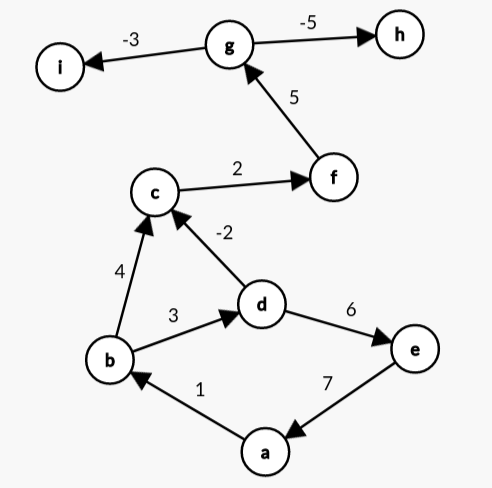
\includegraphics[width=0.8\linewidth]{figs/task-9/graph-9.png}
  \end{minipage}
  \begin{minipage}{0.5\textwidth}
    \centering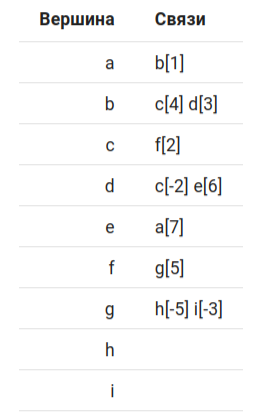
\includegraphics[width=0.6\linewidth]{figs/task-9/adj-9.png}
  \end{minipage}
  \caption{Неориентированный взвешенный граф}
\end{figure}

\begin{minted}{js}
{
  "weighted": true,
  "oriented": true,
  "adj": {
    "a": {
      "b": 1
    },
    "b": {
      "c": 4,
      "d": 3
    },
    "c": {
      "f": 2
    },
    "d": {
      "c": -2,
      "e": 6
    },
    "e": {
      "a": 7
    },
    "f": {
      "g": 5
    },
    "g": {
      "h": -5,
      "i": -3
    },
    "h": {},
    "i": {}
  }
}
\end{minted}

\subsubsection{Выходные данные}
\begin{figure}[H]
  \centering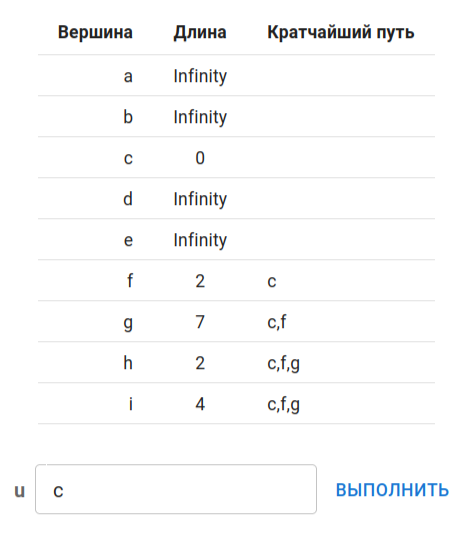
\includegraphics[width=0.6\textwidth]{figs/task-9/res-9.png}
  \caption{Результат работы}
\end{figure}
\section{Веса IV c}
\subsection{Условие задания}
В графе могут быть циклы отрицательного веса.

\textbf{Вариант 10:} Вывести кратчайший путь из вершины $u$ до вершины $v$.

\subsection{Примеры исходного кода}
Для выполнения задания был реализован метод\\
\mitext{taskTen()}:
\begin{minted}{typescript}
/**
 * Метод, который находит кратчайший путь между двумя данными
 * вершинами `u` и `v`. В графе могут быть отрицательные циклы.
 * Реализация построена на алгоритме Флойда.
 * @param u начальная вершина
 * @param v конечная вершина
 */
taskTen(u: string, v: string): { distance: number; path: string[] } {
  if (!this.exists(u)) {
    throw new NodeNotExists(u)
  }
  if (!this.exists(v)) {
    throw new NodeNotExists(v)
  }

  // Map, связывающая строковую метку вершины с числом
  const indexOf = new Map(Array.from(this.adj.keys()).map((v, i) => [v, i]))
  const labelOf = new Map(Array.from(this.adj.keys()).map((v, i) => [i, v]))
  // Список смежности, только метки теперь числа
  const adj = new Map(Array.from(this.adj.entries()).map((v, i) =>
    [i, new Map(Array.from(v[1]).map(v => [indexOf.get(v[0])!, v[1]]))]
  ))
  const vertices = Array.from(adj.keys())

  // инициализировать матрицу расстояний и матрицу следующих вершин
  const dist: number[][] = []
  const next: (number | null)[][] = []

  for (const i of vertices) {
    dist[i] = []
    next[i] = []
    for (const j of vertices) {
      dist[i][j] = i === j ? 0 : Infinity
      next[i][j] = null
    }
  }

  // заполнить матрицу расстояний на основе весов списка смежности
  for (const [src, neighbors] of adj.entries()) {
    for (const [dst, weight] of neighbors.entries()) {
      dist[src][dst] = weight
      next[src][dst] = dst // установить следующую вершину в соответствии с ребром
    }
  }

  // алгоритм Флойда
  for (const k of vertices) {
    for (const i of vertices) {
      for (const j of vertices) {
        if (dist[i][k] + dist[k][j] < dist[i][j]) {
          dist[i][j] = dist[i][k] + dist[k][j]
          next[i][j] = next[i][k]
        }
      }
    }
  }

  // построить кратчайший путь
  if (dist[indexOf.get(u)!][indexOf.get(v)!] >= 0 &&
      dist[indexOf.get(u)!][indexOf.get(v)!] !== Infinity)
  {
    // если в матрице неотрицательное число, значит, вершины
    // не находятся на отрицательном цикле
    const path: string[] = []
    let current = indexOf.get(u) ?? null
    let target = indexOf.get(v)!

    while (current !== target) {
      if (current === null) {
        return {distance: Infinity, path: []}
      }
      path.push(labelOf.get(current)!)
      current = next[current][target]
    }
    path.push(labelOf.get(target)!)

    return {distance: dist[indexOf.get(u)!][indexOf.get(v)!], path}
  }
  else {
    // иначе понятие"кратчайшее расстояние" не существует
    return {distance: -Infinity, path: []}
  }
}
\end{minted}

\subsection{Краткое описание алгоритма}
Этот метод решает задачу нахождения кратчайшего пути между двумя вершинами $u$ и $v$ в графе,
учитывая возможное наличие отрицательных циклов. Реализован на основе алгоритма Флойда.

Создаются отображения \mitext{indexOf} и \mitext{labelOf}, которые связывают строковые метки вершин
с числовыми индексами и наоборот. Также создается матрица смежности \mitext{adj} с числовыми
индексами вершин. Инициализируются матрицы расстояний \mitext{dist} и следующих вершин \mitext{next}.

Заполняется матрица расстояний на основе весов ребер графа. Применяется алгоритм Флойда для нахождения
кратчайших путей между всеми парами вершин в графе.

Строится кратчайший путь от вершины $u$ до вершины $v$ на основе матрицы следующих вершин. Результат
включает в себя длину кратчайшего пути и список вершин, составляющих этот путь.

При отсутствии пути между вершинами $u$ и $v$ в графе возвращается объект с бесконечной длиной пути и
пустым списком вершин.

\subsection{Примеры входных и выходных данных}
\subsubsection{Входные данные}
\begin{figure}[H]
  \begin{minipage}{0.5\textwidth}
    \centering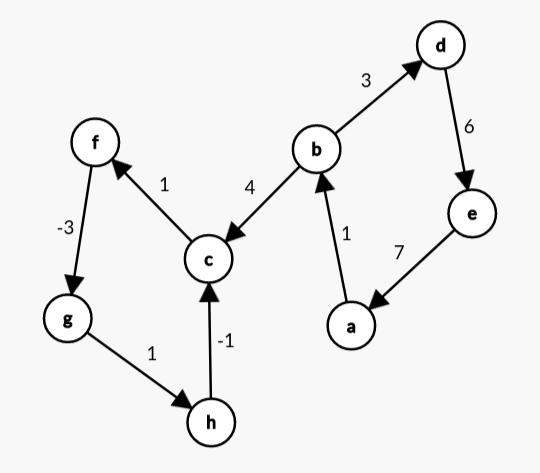
\includegraphics[width=0.8\linewidth]{figs/task-10/graph-10.png}
  \end{minipage}
  \begin{minipage}{0.5\textwidth}
    \centering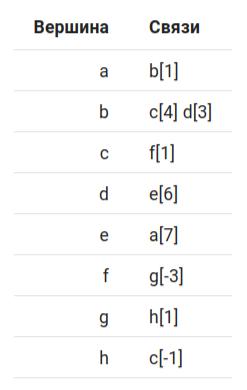
\includegraphics[width=0.5\linewidth]{figs/task-10/adj-10.png}
  \end{minipage}
  \caption{Ориентированный взвешенный граф}
\end{figure}

\begin{minted}{js}
{
  "weighted": true,
  "oriented": true,
  "adj": {
    "a": {
      "b": 1
    },
    "b": {
      "c": 4,
      "d": 3
    },
    "c": {
      "f": 1
    },
    "d": {
      "e": 6
    },
    "e": {
      "a": 7
    },
    "f": {
      "g": -3
    },
    "g": {
      "h": 1
    },
    "h": {
      "c": -1
    }
  }
}
\end{minted}

\subsubsection{Выходные данные}
\begin{figure}[H]
  \begin{minipage}{0.5\textwidth}
    \centering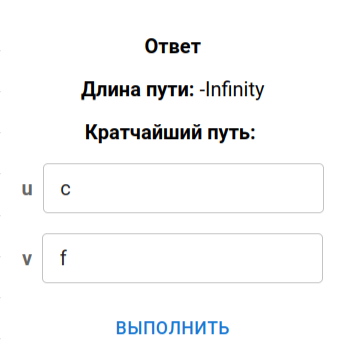
\includegraphics[width=0.7\linewidth]{figs/task-10/res-10-1.png}
  \end{minipage}
  \begin{minipage}{0.5\textwidth}
    \centering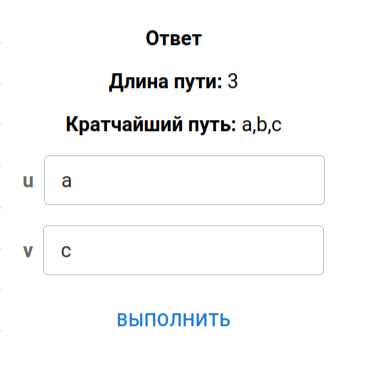
\includegraphics[width=0.7\linewidth]{figs/task-10/res-10-2.png}
  \end{minipage}
  \caption{Результат работы}
\end{figure}
\section{Максимальный поток}
\subsection{Условие задания}
Решить задачу на нахождение максимального потока любым алгоритмом.
Подготовить примеры, демонстрирующие работу алгоритма в разных случаях.

\subsection{Примеры исходного кода}
Для выполнения задания был реализован метод
\mitext{taskEleven()}, а также вспомогательный метод
\mitext{findAugmentingPath()}. С целью экономии места,
код \mitext{findAugmentingPath()} расположен в приложении
\ref{app:max-flow}.
\begin{minted}{typescript}
/**
 * Метод, находящий максимальный поток а графе, используя алгоритм
 * Форда-Фалкерсона.
 * @param source источник
 * @param sink сток
 */
taskEleven(source: string, sink: string): number {
  if (!this.exists(source)) {
    throw new NodeNotExists(source)
  }
  if (!this.exists(sink)) {
    throw new NodeNotExists(sink)
  }

  // создать остаточный граф с теми же вершинами, что и в изначальном
  const resGraph: Map<string, Map<string, number>> = new Map()
  for (const [vertex, edges] of this.adj.entries()) {
    resGraph.set(vertex, new Map(edges))
  }

  let maxFlow = 0

  // расширять поток, пока есть расширяющий путь
  let path = this.findAugmentingPath(resGraph, source, sink)
  while (path.length > 0) {
    // найти минимальную пропускную способность
    const minCapacity = this.findMinCapacity(resGraph, path)

    // обновить остаточный граф вычитанием минимальной пропускной способности
    for (let i = 0; i < path.length - 1; i++) {
      const u = path[i]
      const v = path[i + 1]

      resGraph.get(u)!.set(v, resGraph.get(u)!.get(v)! - minCapacity)

      // добавить обратную дугу с отрицательным весом
      if (!resGraph.has(v)) {
        resGraph.set(v, new Map())
      }

      if (!resGraph.get(v)!.has(u)) {
        resGraph.get(v)!.set(u, 0)
      }

      resGraph.get(v)!.set(u, resGraph.get(v)!.get(u)! + minCapacity)
    }

    // обновить значение максимального потока
    maxFlow += minCapacity

    // найти максимальный расширяющий путь
    path = this.findAugmentingPath(resGraph, source, sink)
  }

  return maxFlow
}
\end{minted}

\subsection{Краткое описание алгоритма}
Создается остаточный граф, который изначально совпадает с оригинальным графом,
но все веса обратных ребер устанавливаются в 0.

Алгоритм производит поиск расширяющих путей в остаточном графе с помощью вспомогательного
метода \mitext{findAugmentingPath()}. Этот метод использует обход в ширину (BFS) для нахождения
пути от источника к стоку, учитывая только те ребра, у которых остаточная пропускная способность больше нуля.

Если найден расширяющий путь, вычисляется минимальная пропускная способность на этом пути. Затем
обновляются значения остаточных пропускных способностей вдоль этого пути путем вычитания минимальной
пропускной способности.

Процесс поиска расширяющих путей и их обновления в остаточном графе повторяется до тех пор, пока не
удастся найти больше расширяющих путей. В процессе выполнения алгоритма суммируется пропускная
способность всех найденных путей, что и является максимальным потоком.

\subsection{Примеры входных и выходных данных}
\subsubsection{Входные данные}
Простой граф с двумя вершинами и одним направленным ребром.
\begin{figure}[H]
  \begin{minipage}{0.5\textwidth}
    \centering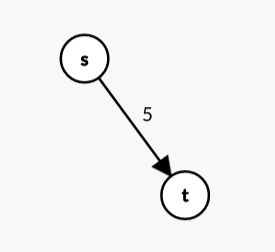
\includegraphics[width=0.6\linewidth]{figs/task-11/graph-ff-1.png}
  \end{minipage}
  \begin{minipage}{0.5\textwidth}
    \centering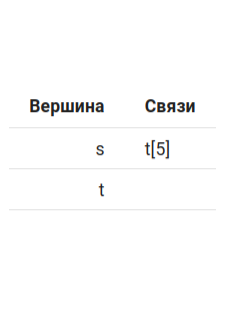
\includegraphics[width=0.6\linewidth]{figs/task-11/adj-ff-1.png}
  \end{minipage}
  \caption{Ориентированный взвешенный граф}
\end{figure}

\begin{minted}{js}
{
  "weighted": true,
  "oriented": true,
  "adj": {
    "s": {
      "t": 5
    },
    "t": {}
  }
}
\end{minted}

\subsubsection{Выходные данные}
\begin{figure}[H]
  \centering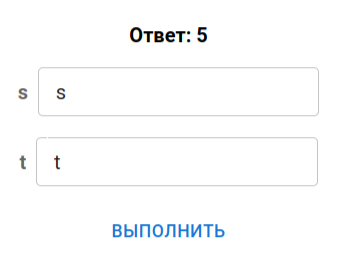
\includegraphics[width=0.3\textwidth]{figs/task-11/res-ff-1.png}
  \caption{Результат работы}
\end{figure}

\subsubsection{Входные данные}
Более сложный граф с четырьмя вершинами и несколькими ребрами.
\begin{figure}[H]
  \begin{minipage}{0.5\textwidth}
    \centering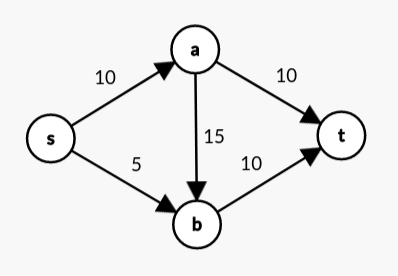
\includegraphics[width=0.8\linewidth]{figs/task-11/graph-ff-2.png}
  \end{minipage}
  \begin{minipage}{0.5\textwidth}
    \centering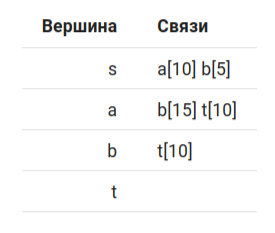
\includegraphics[width=0.6\linewidth]{figs/task-11/adj-ff-2.png}
  \end{minipage}
  \caption{Ориентированный взвешенный граф}
\end{figure}

\begin{minted}{js}
{
  "weighted": true,
  "oriented": true,
  "adj": {
    "source": {
      "a": 10,
      "b": 5
    },
    "a": {
      "b": 15,
      "sink": 10
    },
    "b": {
      "sink": 10
    },
    "t": {}
  }
}
\end{minted}

\subsubsection{Выходные данные}
\begin{figure}[H]
  \centering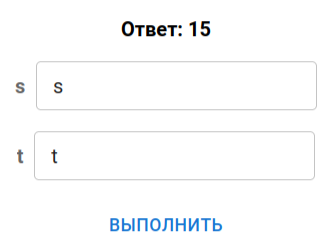
\includegraphics[width=0.3\textwidth]{figs/task-11/res-ff-2.png}
  \caption{Результат работы}
\end{figure}

\subsubsection{Входные данные}
\begin{figure}[H]
  \begin{minipage}{0.5\textwidth}
    \centering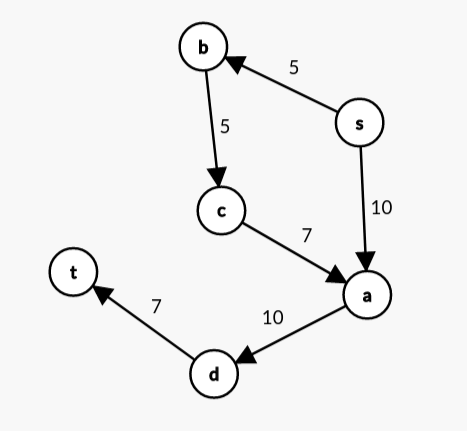
\includegraphics[width=0.8\linewidth]{figs/task-11/graph-ff-3.png}
  \end{minipage}
  \begin{minipage}{0.5\textwidth}
    \centering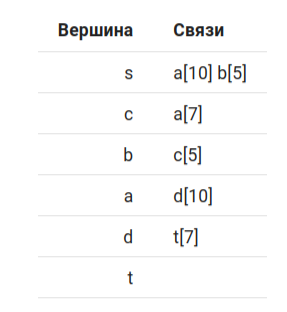
\includegraphics[width=0.6\linewidth]{figs/task-11/adj-ff-3.png}
  \end{minipage}
  \caption{Ориентированный взвешенный граф}
\end{figure}

\begin{minted}{js}
{
  "weighted": true,
  "oriented": true,
  "adj": {
    "s": {
      "a": 10,
      "b": 5
    },
    "c": {
      "a": 7
    },
    "b": {
      "c": 5
    },
    "a": {
      "d": 10
    },
    "d": {
      "t": 7
    },
    "t": {}
  }
}
\end{minted}

\subsubsection{Выходные данные}
\begin{figure}[H]
  \centering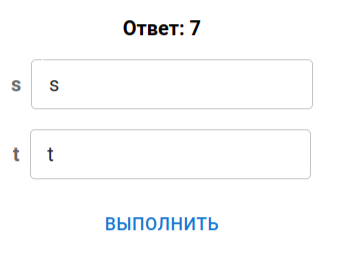
\includegraphics[width=0.3\textwidth]{figs/task-11/res-ff-3.png}
  \caption{Результат работы}
\end{figure}

\conclusion
В ходе практики был выполнен ряд задач, которые поспособствовали закреплению
и углублению теоретических знаний по дисциплине <<Теория графов>>, посредством
реализации класса <<Граф>> на языке TypeScript.

\inputencoding{cp1251}
\bibliographystyle{gost780uv}
\bibliography{thesis}
\inputencoding{utf8}

% Окончание основного документа и начало приложений Каждая последующая секция
% документа будет являться приложением
\appendix
\section{Компонент \mitext{App} веб"=интерфейса}
\label{app:app-component}

\begin{minted}{jsx}
function App() {
  const graph = useRef(new Graph(false, false))
  const [newNode, setNewNode] = useState<string>('')
  const [deleteNode, setDeleteNode] = useState<string>('')
  const [connNodeA, setConnNodeA] = useState<string>('')
  const [connNodeB, setConnNodeB] = useState<string>('')
  const [connNodeWeight, setConnNodeWeight] = useState<number | null>(null)
  const [delConnA, setDelConnA] = useState<string>('')
  const [delConnB, setDelConnB] = useState<string>('')
  const [shouldRerender, setShouldRerender] = useState<boolean>(true)

  const orientedSelection = useRef('unoriented')
  const weightedSelection = useRef('non-weighted')

  useEffect(() => {
      setShouldRerender(false)
    }, [shouldRerender]
  )

  function onCreateNodeClick() {
    if (!newNode) {
      alert('Незаполненные поля!')
      return
    }

    try {
      graph.current.addNode(newNode)
    }
    catch (e) {
      if (e instanceof GraphError) {
        alert(e.message)
        return
      }
    }
    setNewNode('')
    setShouldRerender(true)
  }

  function onDeleteNodeClick() {
    if (!deleteNode) {
      alert('Незаполненные поля!')
      return
    }

    try {
      graph.current.removeNode(deleteNode)
    }
    catch (e) {
      if (e instanceof GraphError) {
        alert(e.message)
        return
      }
    }
    setDeleteNode('')
    setShouldRerender(true)
  }

  function onConnectNodesClick() {
    if (!connNodeA || !connNodeB || (graph.current.isWeighted() && !connNodeWeight)) {
      alert('Незаполненные поля!')
      return
    }

    try {
      graph.current.connect(connNodeA, connNodeB, connNodeWeight ?? undefined)
    }
    catch (e) {
      if (e instanceof GraphError) {
        alert(e.message)
        return
      }
    }
    setConnNodeA('')
    setConnNodeB('')
    setConnNodeWeight(null)
    setShouldRerender(true)
  }

  function onDeleteConnectionClick() {
    if (!delConnA || !delConnB) {
      alert('Незаполненные поля!')
      return
    }

    try {
      graph.current.disconnect(delConnA, delConnB)
    }
    catch (e) {
      if (e instanceof GraphError) {
        alert(e.message)
        return
      }
    }
    setDelConnA('')
    setDelConnB('')
    setShouldRerender(true)
  }

  function onGraphLoaded(fileContent: string) {
    try {
      graph.current = new Graph(fileContent)
    }
    catch (e) {
      alert('Неверный формат файла!')
      return
    }

    if (graph.current.isOriented()) {
      orientedSelection.current = 'oriented'
    }
    else {
      orientedSelection.current = 'unoriented'
    }

    if (graph.current.isWeighted()) {
      weightedSelection.current = 'weighted'
    }
    else {
      weightedSelection.current = 'non-weighted'
    }

    setShouldRerender(true)
  }

  function onGraphOrientedChange(value: string) {
    orientedSelection.current = value
    graph.current.changeOriented(value === 'oriented')
    setShouldRerender(true)
  }

  function onGraphWeightedChange(value: string) {
    weightedSelection.current = value
    graph.current.changeWeighted(value === 'weighted')
    setShouldRerender(true)
  }

  return (
    <div id='app'>
      <header>
        <h2>Взаимодействие с графом</h2>
      </header>
      <div className='controls'>
        <div className='control' style={{ gridColumnStart: '2', gridColumnEnd: '4' }}>
          <InputLabel>Ориентированность</InputLabel>
          <Select value={orientedSelection.current}
                  onChange={e => onGraphOrientedChange(e.target.value)}>
            <MenuItem value='unoriented'>Неориентированный</MenuItem>
            <MenuItem value='oriented'>Ориентированный</MenuItem>
          </Select>
        </div>
        <div className='control' style={{ gridColumnStart: '4', gridColumnEnd: '6' }}>
          <InputLabel>Взвешенность</InputLabel>
          <Select value={weightedSelection.current}
                  onChange={e => onGraphWeightedChange(e.target.value)}>
            <MenuItem value='weighted'>Взвешенный</MenuItem>
            <MenuItem value='non-weighted'>Невзвешенный</MenuItem>
          </Select>
        </div>
        <div className='control' style={{gridTemplateColumns: '1fr 1fr 1fr', gridColumnStart: '2', gridColumnEnd: '6'}}>
          <GraphLoader onGraphLoaded={onGraphLoaded} />
          <GraphDumper graph={graph} />
        </div>
        <div className='control' style={{gridColumnStart: '2', gridColumnEnd: '4'}}>
          <InputLabel>Создать узел</InputLabel>
          <TextField value={newNode ?? ''}
                     type='text'
                     onChange={e => setNewNode(e.target.value)}
                     size='small'>
          </TextField>
          <Button onClick={onCreateNodeClick}>Добавить</Button>
        </div>
        <div className='control' style={{gridColumnStart: '4', gridColumnEnd: '6'}}>
          <InputLabel>Удалить узел</InputLabel>
          <TextField value={deleteNode ?? ''}
                     type='text'
                     onChange={e => setDeleteNode(e.target.value)}
                     size='small'>
          </TextField>
          <Button onClick={onDeleteNodeClick}>Удалить</Button>
        </div>
        <div className='control' style={{gridColumnStart: '2', gridColumnEnd: '4'}}>
          <InputLabel>Соединить узлы</InputLabel>
          <div style={{ display: 'grid', gridTemplateRows: '1fr 1fr 1fr'}}>
            <TextField value={connNodeA ?? ''}
                       type='text'
                       onChange={e => setConnNodeA(e.target.value)}
                       size='small'
                       style={{paddingBottom: '0.5em'}}>
            </TextField>
            <TextField value={connNodeB ?? ''}
                       type='text'
                       onChange={e => setConnNodeB(e.target.value)}
                       size='small'
                       style={{paddingBottom: '0.5em'}}>
            </TextField>
            <TextField value={connNodeWeight ?? ''}
                       type='number'
                       onChange={e => setConnNodeWeight(Number(e.target.value))}
                       size='small'>
            </TextField>
          </div>
          <Button onClick={onConnectNodesClick}>Соединить</Button>
        </div>
        <div className='control' style={{gridColumnStart: '4', gridColumnEnd: '6'}}>
          <InputLabel>Удалить связь</InputLabel>
          <div style={{ display: 'grid', gridTemplateRows: '1fr 1fr'}}>
            <TextField value={delConnA ?? ''}
                       type='text'
                       onChange={e => setDelConnA(e.target.value)}
                       size='small'
                       style={{paddingBottom: '0.5em'}}>
            </TextField>
            <TextField value={delConnB ?? ''}
                       type='text'
                       onChange={e => setDelConnB(e.target.value)}
                       size='small'>
            </TextField>
          </div>
          <Button onClick={onDeleteConnectionClick}>Удалить</Button>
        </div>
      </div>
      <main style={{width: '100%', display: 'flex', justifyContent: 'center'}}>
        <div id='connections'>
          <GraphView graph={graph} />
        </div>
      </main>
      <hr />
      <div id='tasks'>
        <TaskOne />
        <hr />
        <!-- Остальные компоненты задач -->
      </div>
    </div>
  )
}
\end{minted}
\section{Дополнительный код к заданию <<Максимальный поток>>}
\label{app:max-flow}

\begin{minted}{typescript}
/**
 * Вспомогательный метод, находящий расширяющий путь в
 * остаточном графе, построенный на основе BFS.
 */
private findAugmentingPath(
  residualGraph: Map<string, Map<string, number>>,
  source: string,
  sink: string
): string[] | null {
  const visited: Set<string> = new Set()
  const queue: string[] = [source]
  const parent: Map<string, string | null> = new Map()
  parent.set(source, null)

  while (queue.length > 0) {
    const u = queue.shift()!
    for (const v of residualGraph.get(u)!.keys()) {
      if (!visited.has(v) && residualGraph.get(u)!.get(v)! > 0) {
        visited.add(v)
        parent.set(v, u)
        queue.push(v)

        if (v === sink) {
          // пересоздать расширяющий путь
          const path: string[] = []
          let current = v
          while (current !== null) {
            path.unshift(current)
            current = parent.get(current)!
          }
          return path
        }
      }
    }
  }

  return null // не нашлось расширяющего пути
}
\end{minted}

\end{document}